\documentclass[12pt,fleqn]{article}\usepackage{../../common}
\begin{document}
Materyel, Stress

Gerilme Tensörü (Strain Tensor) 

Önce nesneleri nasıl temsil ettiğimizden bahsedelim. Diyelim ki elimizde bir
patates var. Fakat bu patatesin matematiksel olarak bir anlamı yok. Eğer
bu nesneyi $R^3$ uzayında temsil etmek istiyorsak, onun üzerindeki belli
seçilmiş noktalar sayesinde bunu yapabiliriz.

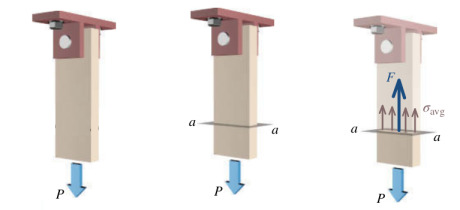
\includegraphics[width=8em]{phy_020_strs_01_01.jpg}

Nesne uzerindeki mavi noktalar bu secilmis noktalari gosteriyor.

Secilmis noktalarin kordinati bir referansa gore alinmali, $e_1,e_2,e_3$
seklinde bir baz bu isi yapabilir. 

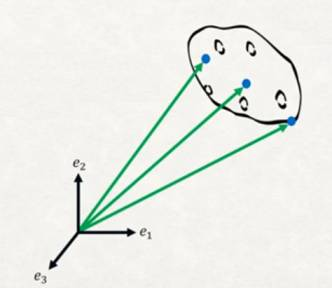
\includegraphics[width=8em]{phy_020_strs_01_02.jpg}



















[devam edecek]

\end{document}
